\anitha{ I am working on the following sections}...
\section{Discussion}




\iffalse
\section{Approach to Automated Traceability}
\label{sec:set-of-support}

prior work - IVC - extension to traceability - evaluation - experiments with multiple set of support.

%\mike{We need to establish the idea of satisfaction arguments between architectural layers prior to this section}
%
%\mike{Check later to determine which parts of this section are redundant}
%
%\mike{Extremely loose use of requirement vs. property.  Nail this down.}
%
%In this section, we describe an approach to use inductive validity cores to construct trace links between different layers in a complex system architecture.

In prior work~\cite{hilt2013}, we demonstrated a model based approach to system construction in which compositional proofs are used to to establish satisfaction arguments. To cope with complexity of modeling and scalability of verification of large systems, we proposed an approach in which systems can be decomposed into subsystems, modeled individually and verified compositionally. Given an architectural model of the system (decomposition of system into components) in which each component (including the system) is endowed with its own set of requirements, we used a tool suite called AGREE~\cite{NFM2012:CoGaMiWhLaLu} -- a reasoning framework based on assume-guarantee reasoning~\cite{McMillan99:circ} -- to compositionally verify whether system level requirements are established as a logical consequence of the component level requirements and the system level assumptions. Using AGREE we were able to verify large and complex systems efficiently. AGREE partitions the task of verification along the architectural lines of the system. Stating from the leaf level, it systematically verifies if the parent level requirements hold as a logical consequence of its immediately child component requirements in the given architecture.

To verify the requirements, AGREE uses a model checker called JKind~\cite{JKIND link}. JKind is an infinite-state model checker that is intended to verify functional requirements, in particular safety requirements. JKind proves safety properties using multiple cooperative engines in parallel including $k$-induction~\cite{SheeranSS00}, property directed reachability~\cite{Een2011:PDR}, and template-based lemma generation~\cite{Kahsai2011}. JKind accepts Lustre programs written over the theory of linear integer and real arithmetic. In the back-end, JKind uses an SMT solver such as Z3~\cite{DeMoura08:z3}, Yices~\cite{Dutertre06:yices}, MathSAT~\cite{Cimatti2013:MathSAT}, or
SMTInterpol~\cite{Christ2012:SMTInterpol}.

The underlying SMT solver automatically tries to constructs proofs to establish satisfaction of requirements in the model. A proof can be visualized as a derivation tree where the leaves of the tree are axioms -- elements of the model such as components requirements, interface connections, system assumptions -- and each interior node represents the application of an inference rule that leads to proving the system requirement. If the solver encounters a violation of a requirement while constructing the proof, it reports it along with a counterexample - a concrete path of execution that explains the violation. On the other hand, when the proof is successfully constructed, the tool reports that the requirement is satisfied. %This approach was able to scalably verify large and complex systems.

%\\begin{figure}[htb]
%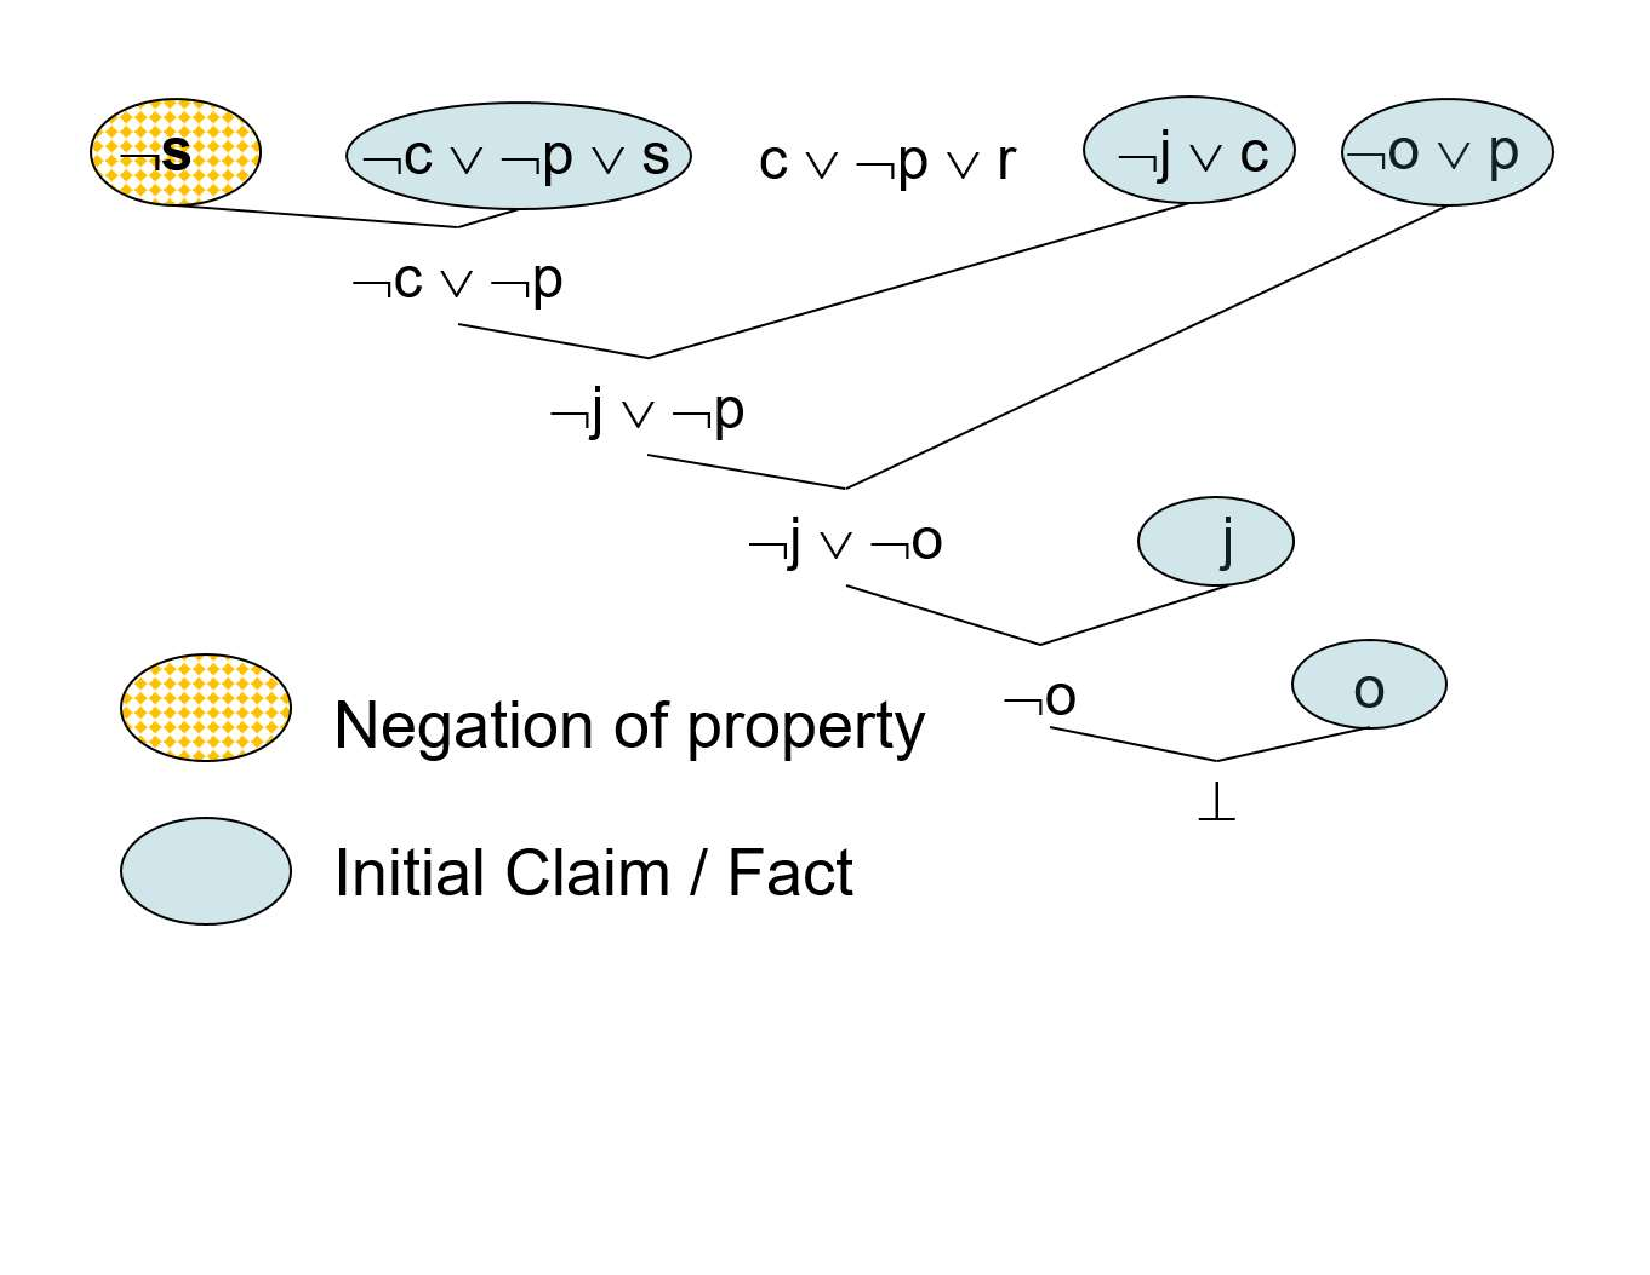
\includegraphics[width=\columnwidth]{images/proof.pdf}
%\mike{This is not accurate w.r.t. JKind actually does for IVCs}
%\caption{An accurate picture would be somewhat difficult.}\label{fig:proof}
%\end{figure}

\subsection{Inductive Invalidity Cores}

While the above approach is very useful in proving system level requirements, in the event
that requirement is proved, it is not always clear what level of assurance should be invested in the
result.  Given that these kinds of analyses are typically performed for safety critical system, this
can lead to overconfidence in the behavior of the fielded system. It is well known that issues such as
vacuity~\cite{Kupferman03:Vacuity} can cause verification to succeed despite errors in a requirements
or in the model. Even for non-vacuous requirements, it is possible to over-constrain the {\em
environment} of the model such that the implementation will not work in the actual operating
environment. Hence, to gain confidence over the verification we pursed an approach that would provide
us with an evidence of the successful verification. An evidence in this context is nothing but an
explanation about which parts of the model (the component requirements and system assumptions) the
model checker used to prove the system level requirement.

Since the solvers typically abstract away the proof it creates, we developed a novel technique to query the solver to excavate the axioms that were used as part of the proof. We call the result to such a query as the {\em inductive validity core} (IVC). The IVC helps explain how the solver reported the satisfaction of the requirement, that is comparable to the counterexample explains the negative result. In general, the IVC extracted is not guaranteed to be contain only the necessary axioms, depending on how the model checker constructed the proof. Hence, in our approach after
extracting the IVC we minimize it by recursively reducing them and checking if the remaining axioms are
the necessary elements for the proof. Further, when induction is involved, many requirements are not
themselves inductively provable and hence proof techniques introduce lemmas as part of the solving
process in order to strengthen those requirements and make them inductive. The novelty of our approach
is its efficient, accurate, and precise extraction of a minimum IVC in the presence of such auxiliary
lemmas.

Extracting the IVC was a significant step towards testing our hypothesis, but it was not sufficient, since the IVCs were not in a easily understandable format. In the process of verifying the requirements AGREE, JKind and the underlying solvers transform the original model into a number of intermediate models that no longer resemble the original model. The IVCs were parts of the transformed model that was not directly correlatable to the original model. Hence, to be understandable, the IVCs had to be linked back to parts of the original model. This was critical for establishing traceability that is meaningful. In the next subsection, we explain our approach to rigorously link the IVC to actual parts of the model to establish traceability between the requirements and the model.

\subsection{Automated Traceability}

\begin{figure}[htb]
\begin{center}
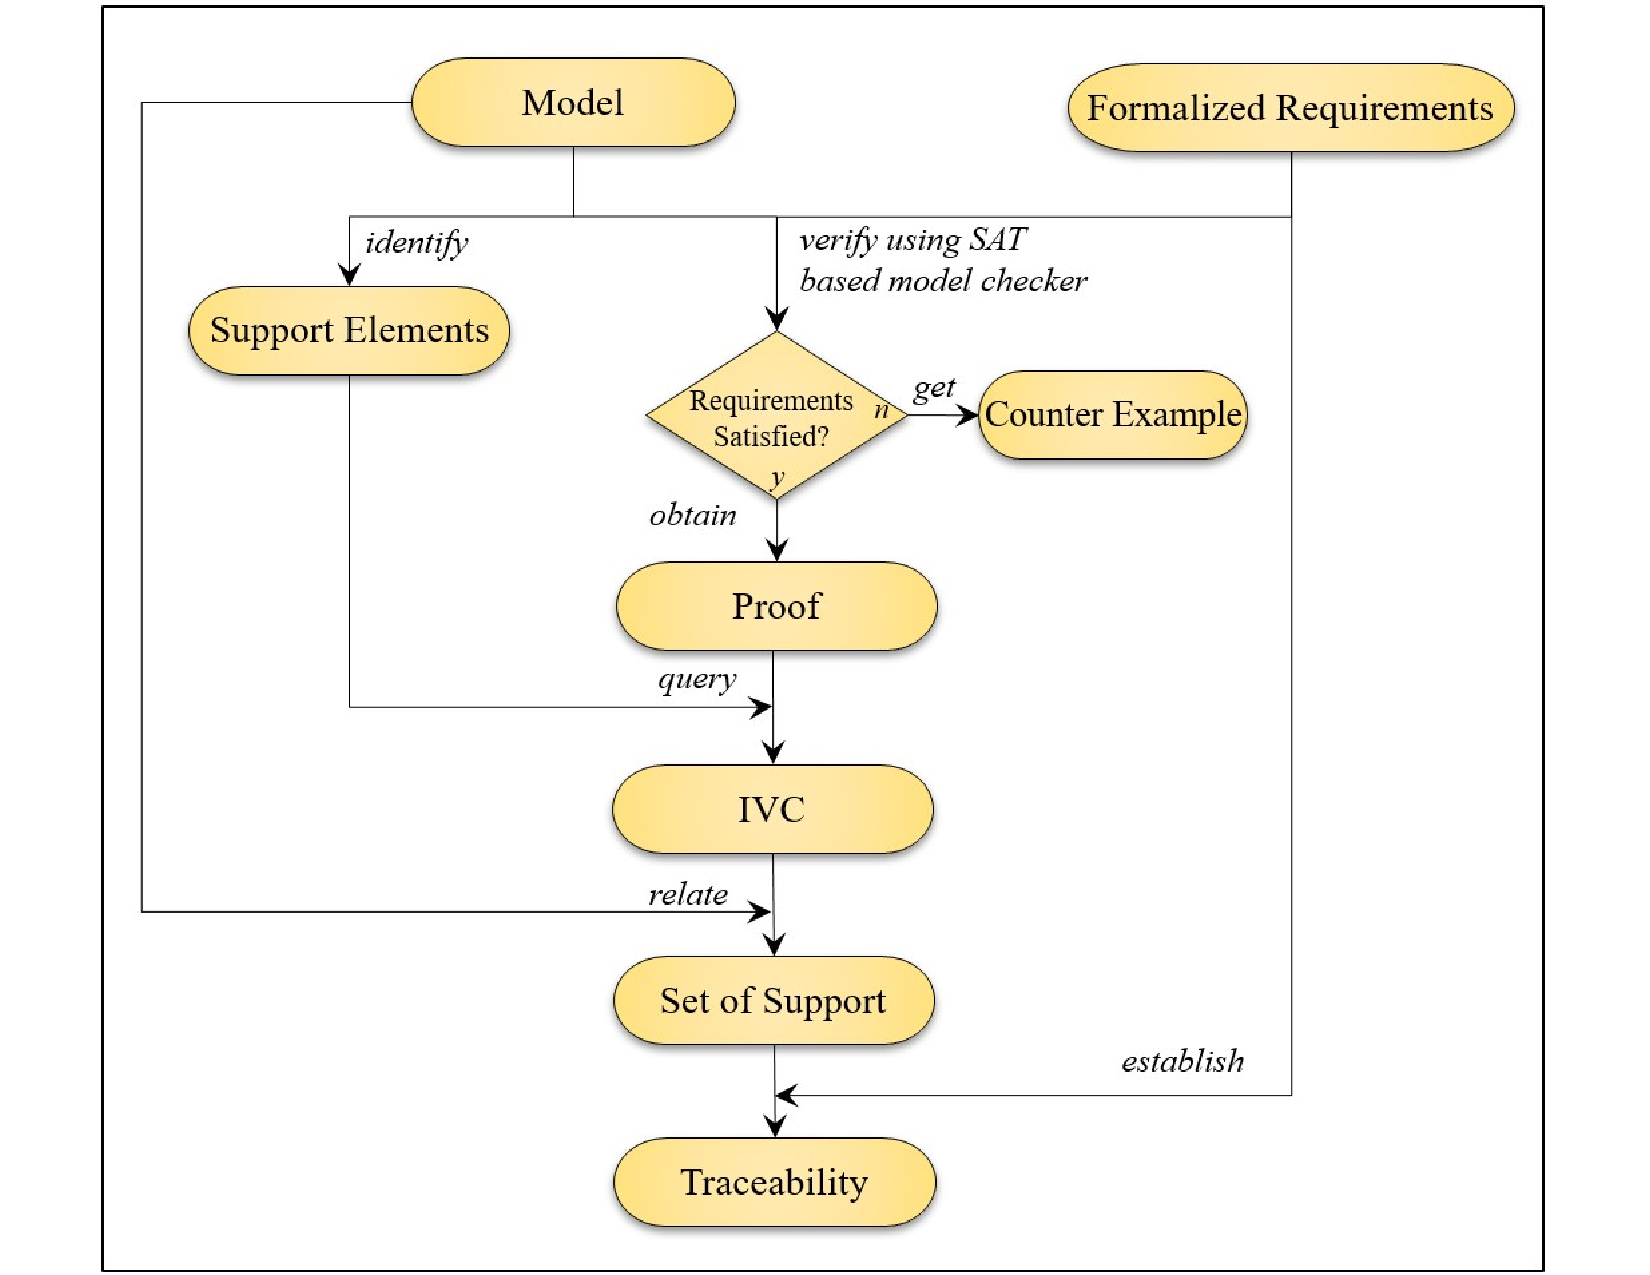
\includegraphics[width=\columnwidth]{images/approach.pdf}
\caption{Approach to Automated Traceability}\label{fig:approach}
\end{center}
\end{figure}

The approach requires two inputs: the architectural model of the system specified in AADL and the formalized requirements in the AGREE formalism, as shown in Figure~\ref{fig:approach}. The parts of the model that one wants to trace to the requirements are identified and marked. We call them \emph{support elements}. While one could systematically identify all parts of the model as support elements, we believe that not every part of the model is interesting to trace depending upon the type of the model. Once the support elements are identified, the model verified with respect to a set of formalized requirements using a SMT based model checker. If a property is not valid, the model checker returns a counterexample that can then be used for debugging the issue.  If a property is satisfied, the solver is queried to check which of the model elements were used by the solver to construct the proof of satisfaction for that requirement.  This set of elements returned by the solver is called an Inductive Validity Core (IVC) described in Section~\ref{sec:background}.  In order to use the IVC for traceability, it is necessary to map it back to the elements of the original model. We refer to these elements as the {\em set of support} for the requirement.

To implement our approach, we extended the AGREE tool in such a way that the users are provided with an option to choose to establish traceability as they verify the requirements. To enable traceability, we changed the way AGREE tool parses the AADL model, so that it can automatically identify and marked all the relevant parts of the model as support elements (as mentioned earlier we marked the system level assumptions and component requirements). Once the support elements are identified, the underlying solver verifies if the requirements is satisfied and returns the IVC. To map the IVC back to original model parts, we had to create references to the model and persist them throughout the process, that involved a significant engineering effort. Once mapped the set of support elements are displayed to the user for every verified requirement.

\subsection{Evaluation}
\anitha{may be we dont need a subsection. But I wanted to show some results}
%\anitha{I am discussing GPCA example here. Do we want a table with other models and their properties proved?}
%\mike{Why?  This is not an experiment; it is simply an exemplar}.


\begin{figure}[htb]
\begin{center}
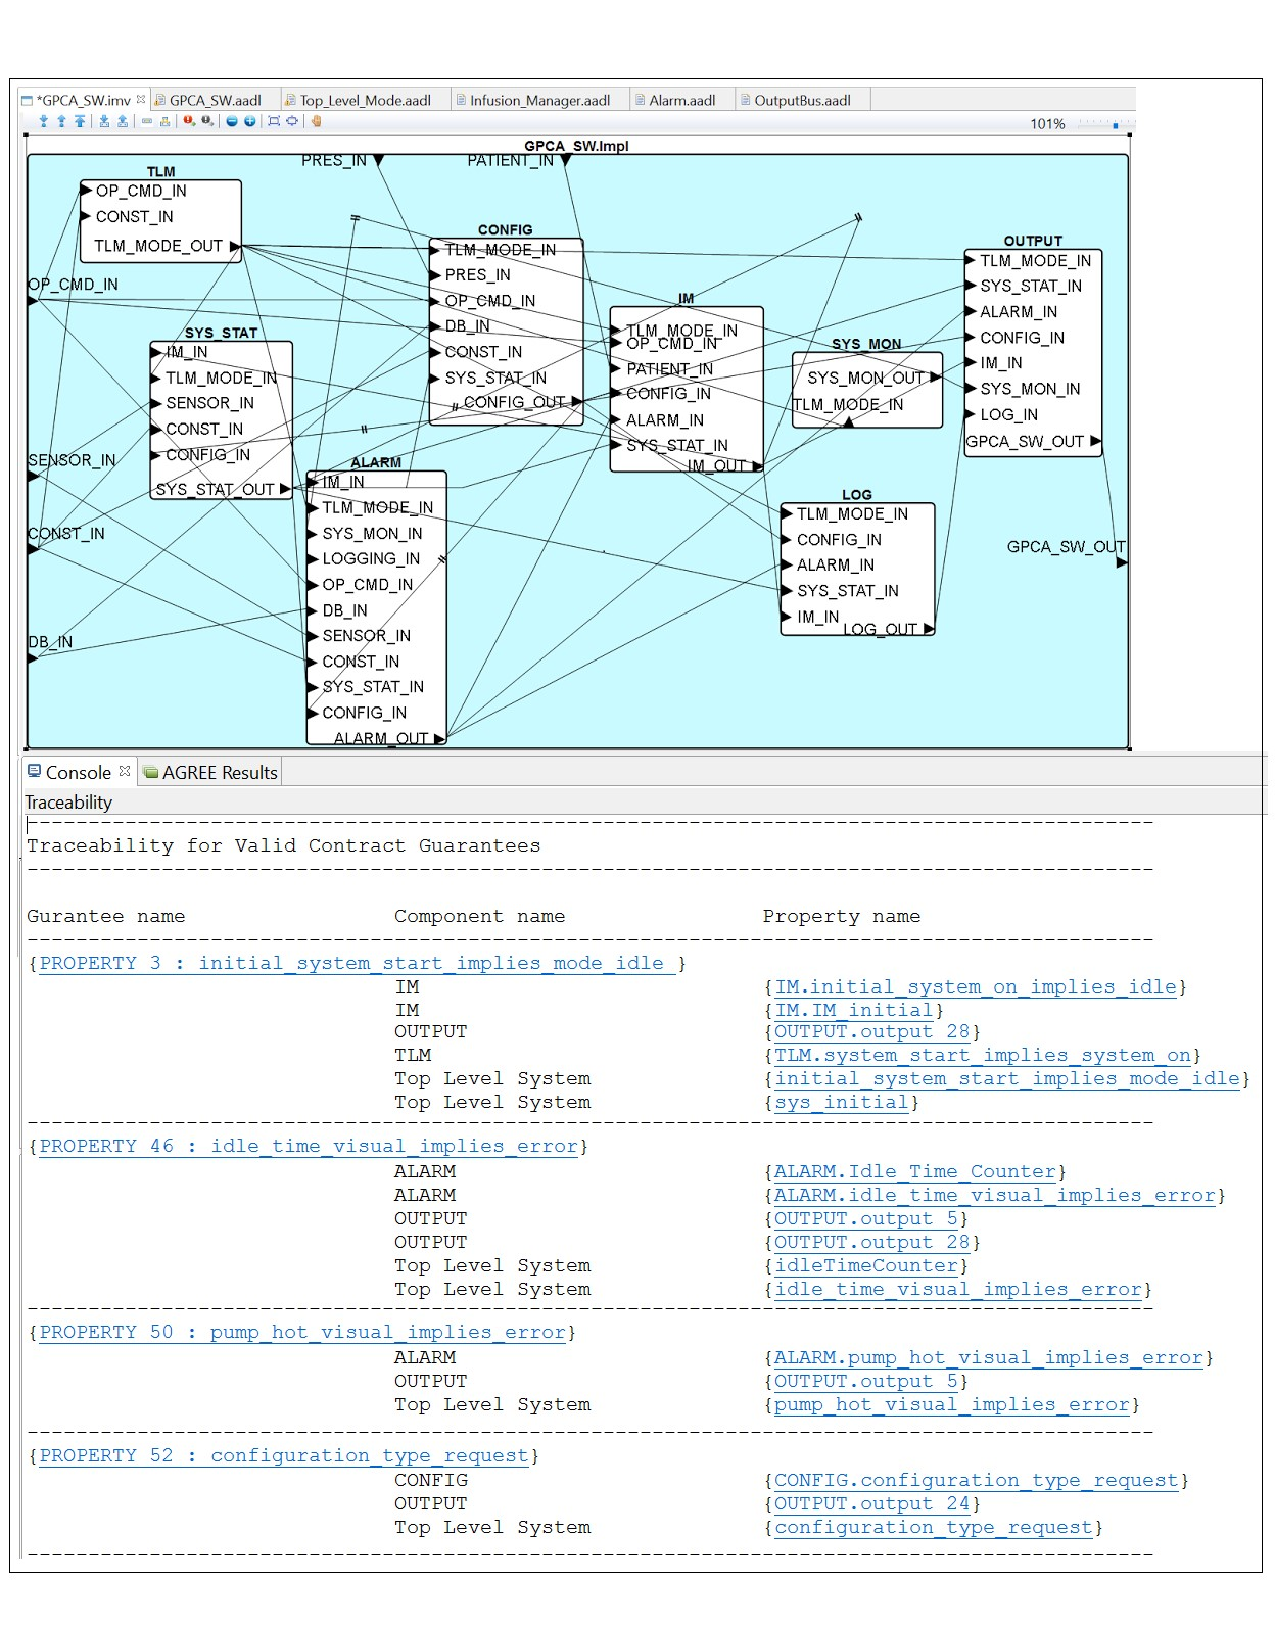
\includegraphics[width=\columnwidth]{images/gpca.pdf}
\caption{Architectural Model and Traceability of Infusion Pump}\label{fig:gpca}
\end{center}
\end{figure}

To evaluate our approach, we used a substantially complex model of a medical device system, the software of an infusion pump. To cope with complexity, the infusion pump was decomposed into 8 components, each allocated with own set of requirements. The Figure shows the architectural model of the infusion pump. The infusion pump had 56 system level requirements, 7 system level assumptions and a total of 120 component level requirements. Our approach was able to successfully verify and establish traceability between each of the system level requirement and its set of support - the component level requirements and system level assumptions that were necessary for its satisfaction. The tool took 89 seconds for both verifying and establishing trace links for the infusion pump system. We believe that this was enormously useful since the traceability was precise and as well as fully automated. Whenever there was a change to the requirement or model one could automatically re-establish the trace links. The Figure shows the tool displays the traceability information. We also made each element in the set of support as clickable so that one can easily navigate to the actual location of that support element in the model.

In an attempt to compare the way traceability is established manually and by our approach, we asked the developer, who formalized the requirements and verified them in the tool, to manually record the trace links between the system level and component requirements. This activity lead to a couple of interesting observations about the way traceability was recorded. First of all, there was a significant difference in the elaborateness of the traces. The developer recorded only those component requirements that were significant to satisfying the requirement. On the other hand, our approach identified all those component requirements that were necessary to establish a satisfaction argument. Although one could argue that tracing to all necessary component requirements is not required (since one might think some of them are insignificant), in our experience we found that to perform rigorous analysis, say impact of a requirement change, traceability to all the necessary requirements was crucial. Another interesting observation is the difference in precision of recording the trace. For one of the system requirements, the developer traced to a component requirement that was allocated inorder to to satisfy that system requirement. However, our approach returned a system level assumption as its set of support. This indicated that the requirement was vacuously satisfied due to a over constrained environment rather than by the component. This helped us fix the error in the assumption. Hence, it was evident that our approach to traceability was much precise than the one that was manually documented.

\subsection{Complete Traceability}


\fi 